% Chapter Template

\chapter{Related Work} % Main chapter title

\label{Chapter 2} % Change X to a consecutive number; for referencing this chapter elsewhere, use \ref{ChapterX}

\lhead{Chapter 2. \emph{Related Work}} % Change X to a consecutive number; this is for the header on each page - perhaps a shortened title

%----------------------------------------------------------------------------------------
%	SECTION 1
%----------------------------------------------------------------------------------------

%\section{State of the Art}

\section{Overview}

Over the last two decades, the focus of the Machine Learning community on deep learning, (ie the study of Deep Neural Networks) has grown considerably. Because of the hardware improvements as well as several improvement of the optimization techniques, Neural Networks outperforms other Machine Learning techniques in many domains and applications where they have won several competitions. Escpecially when it concerns problems with large set of input features or complex sequential relations (for instance in Computer Vision, or voice recognition). It is therefore natural to use the approach of training a Recurrent Neural Network to learn the music representation as this approach has been sucessful in solving similar problems. In the following, we will detail some of the achievements and techniques used with Neural Networks to motivate and justify this choice. The recent survey paper of Schmidhuber et al. \cite{schmidhuber2014deep} and Bengio et al.\cite{bengio2013advances} was very useful in the orientation of the relevant related work. 

\newpage
\section{Recurrent Neural Network}

Artificial Neural Networks (ANNs) were introduced in the 1940s (e.g., McCulloch and Pitts, 1943) in an attempt to model the functionning of the brain, even if the first models are inspired of linear regression introduced by mathematicians like Gauss and Legendre in the 19th centery. An artificial neural network contains a graph, where the nodes are representing neurons. A neuron can be an input neuron, directly connected to an input from a sensor or a dataset, a hidden neuron with different inputs from other neurons or an output neuron, also with different inputs from neurons, but from which it is possible to read a value. Different models have been built to model the interaction between neurons. These models can be inspired directly from biology (for instance in the hodgkin-huxley model \cite{lytton2002hodgkin}). For the specific use of Machine Learning problems however, the model of the neurons is simplified to be able to use large networks of neurons and the backpropagation algorithm. The classical form of the neuron is as follow : 
$$ out = a (W * X + b)$$ where, $W$ it the weight matrix and $b$ a bias vector. $a$ is called the activation function and can be used to introduce non-linearity in the model.
Classical activation functions have sigmoid shape like hyperbolic tangent or the logistic function ($ \frac 1 {1 + \exp x}$).
Lately however the use of rectified linear unit (ReLU): $$a(x) = max(x, 0)$$ have shown significant improvement for some applications (mainly for calculation speed reasons \cite{dahl2013improving})  
It is possible to use this equation to update a set of neurons directly and simplify the notation using matrix notations. 

The model of the Feedforward Neural Networks (FNN), with no recurrent connection (ie no loops) can be described as follow:

$$
\begin{array}{rcr} 
    h_0 & = & x \\h_i & = & a ( W_{i} * h_{i-1}) \\ \hat{y} & = & h_n
\end{array}
$$

where the set of neurons is organised in layer ($n$ is the number of layers and $h_i$ is the output of the $i_{th}$ layer ). The shapes of the weight matrix $W_i$ describe the topology of the graph of neurons, ie the architecture of neural network. FNNs are an improvement of the logistic regression model (a network with 1 layer). It is possible to learn the weights matrices and biases using gradient descent. The success of the FNN model comes from the backpropagation algorithm, witch enables to compute the gradient of the error of the model  $error = D(y, \hat{y})$ where D is a distance function between the prediction of the network and the real value to be predicted. The gradient is computed over the set of parameters (ie the weights and biases) efficiently using the function composition gradient (backward propagation of the error).

A Recurrent Neural Network (RNN) is a more general type of network where loops in the connection are allowed. Because of the loops, it is not possible to use the backpropagation algorithm in the same way as for Feedforward Neural Networks. For the same reason it is convenient to introduce a time dependency in RNNs (some neurons may have states that don't converge). The equation describing a Recurrent Neural Network can be written as follow : 


Given a sequence of inputs: $x_1, x_2, ... x_t$ and the hidden states $h_1, h_2, ..., h_t$.
$$
\begin{array}{rcr} 
    h_0 & = & a(W_{hx}  * x_0 + b_{init} + b_h)  \\ 
    h_i & = & a(W_{hx}  * x_i + W _{hh} * h_{i-1} + b_h)  \\ 
    \hat{y}_i & = & a'(W_{yh} + b_y)

\end{array}
$$

\begin{figure}[htbp]
    \centering
    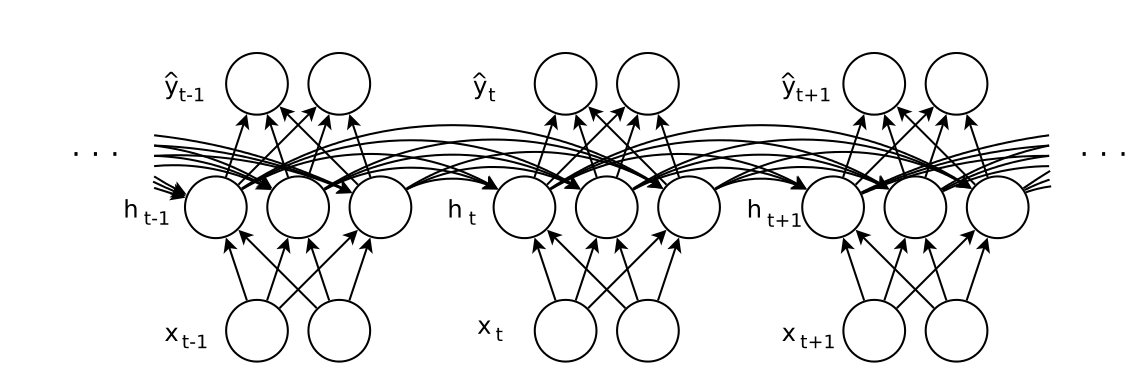
\includegraphics[scale=0.3]{Figures/RNN.png}
    \rule{35em}{0.5pt}
    \caption[Recurrent Neural Network]{Recurrent Neural Network}
    \label{fig:rnn}
\end{figure}




We generate a set of predictions ($\hat{y}_1, \hat{y}_2, ... \hat{y}_t$) from the network. The architecture is described with the shapes of the weight matrix $W_{hx}$ (input to hidden), $W_{hh}$ (hidden to hidden) and $W_{yh}$ (hidden to output). The parameters of the network are the weights and the biases ($b_h$, $b_{init}$, $b_y$).
We can consider this network as a special kind of very deep Feed Forward Network, where each time step has its own layer and with constraints on the weights. With this analogy it is possible to build a version of the backpropagation algorithm for Recurrent Neural Networks called Backpropagation trough time \cite{werbos1990backpropagation}.


\section{Hessian Free Optimization}

Efficiently training a Neural Network remains an area of focus of the Machine Learning community. In the 1990s, this problem seemed impossible to solve for real applications and many machine learning researcher prefered other methods. In the last decade, the progress of computation power, as well as implementation of fast matrix calculation on Graphics Processing Units (GPU) made it possible for neural network to be trained much faster. But the progress of computation is not the only reason for the sucess of Neural Networks today. Many improvements in the model, such as Hinton et al. dropouts \cite{dahl2013improving}, implementation of convolutional neural network on GPU \cite{krizhevsky2012imagenet} or the introduction of Long Short Term Memory Recurrent Neural Networks (LSTM, hochreiter et al. \cite{hochreiter1997long}) and on the optimization method where introduced. One of the major issue with standard stochastic gradient descent when applied to deep Neural Networks, and therefore to Recurrent Neural Networks is the called exploding vanishing gradient. When evaluating the gradient of the error of the network on the weight, because of the derivative of the composition of 2 functions, products of weights appear in the calculations of the gradient. When the network is deep, is can be shown that this product of weights grows exponentially \cite{pascanu2012difficulty}. The difference between the gradient on different direction in the parameters space makes it harder for the gradient descent to converge. To undestand this phenomena, we can consider the gradient descent applied to a problem where the equipotential are flat ellipses. The direction given by the gradient will be toward the largest axis of the elipse, and it will take many steps to converge toward the center of the elipse. In the opposite if the equipotential is a circle, then the direction given by the gradient is the best. 


\begin{figure}[htbp]
    \centering
    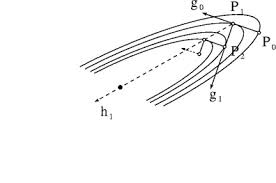
\includegraphics[scale=0.7]{Figures/gradient_ellipse.jpg}
    \rule{35em}{0.5pt}
    \caption[Difficulty of gradient descent]{Difficulty of gradient descent}
    \label{fig:gradient_elipse}
\end{figure}

In order for the gradient direction to be less dependant to linear transformation of the parameter space, we need to look at higher order of derivatives. Applying newton's method to $\phi(X)$ is the same as applying it to $\phi(A*X)$ for $A$ invertible. However, newton's method requires to inverse the curvature matrix, which is not computationally feseable, event for medium size networks. Several techniques used in optimization perform lower rank approximation (L-BFGS) of the curvature matrix in order to solve this issue. However, these approximations are not satisfactory for deep neural networks, because the approximation will be to influenced by the exploding and vanishing gradient. In 2010, Martens et al. proposed several modification to the Hessian Free Optimization techniques in order to apply them to Deep Neural Networks \cite{martens2010deep} and to Recurent Neural Networks \cite{martens2011learning}. 

The Hessian Free Optimization method, like the gradient descent is an iterative process. It takes into account the curvature (ie the second order derivative) of the fitness function, but does not require the inversion of the matrix nor any approximation of the curvature. At each step, in order to get the next iteration point, the hessian matrix is calculated and the conjugate gradient descent is applied to the sum of the second order approximation of the fitness function at this point and a damping function, ie minimize:
$$ q\theta_n = M\theta_n(\theta) + \lambda * R\theta_n(\theta) $$

where the second order approximation of the fitness function is $$M\theta_n (\theta) = f(\theta) + f'(\theta_n)^\top * (\theta  - \theta_n)+ (\theta - \theta_n)^\top * B * (\theta - \theta_n) $$ and $\lambda * R(\theta_n)$. Among other modifications, Martens et al. proposed to replace the curvature matrix B with the Gauss-Newton curvature matrix (which is semi-definite) as well as proposing a specific term for the specific case of Recurrent Neural Networks \cite{martens2011learning}.
The Hessian Free Optimization method then uses conjugate gradient descent to minimize the second order approximation $q\theta_n(\theta)$. It is not necessary to wait for the full convergence of the Conjugate Gradient descent, as the precised minimum of the second order is not relevant, however, Martens et al proposed a condition to stop the convergence and go the next step.


\section{Text and Polyphonic Music Generation using Recurrent Neural Networks}

Sutskever et al. \cite{sutskever2011generating} applied a recurrent neural network using the Hessian Free Optimization method to learn a representation of natural language. Sutskever trained the network on Wikipedia character strings to predict the next character. In this work, the generative properties of the Neural Network were used to produce text. By feeding the prediction of the network as the last character of its input string, it is possible to generate sentences. The character is found using a standard softmax function. The generated text presented really interesting patterns of natural language even at a character level, such as vocabulary and syntax, as well as learning opening and closing brackets. Here is a sample of the generated Text, that used "The meaning of life is" as it starting string: 

\begin{quote}
The meaning of life is the tradition of the ancient human reproduction: it is less favorable to the good boy for when to remove her bigger. In the show’s agreement unanimously resurfaced. Thewild pasteured with consistent street forests were incorporated by the 15th century BE.
\end{quote}

Boulanger-Lewandowski et al. worked on appying recurrent neural networks as well as using probabilistic models to generate polyphonic music from symbolic scores of music\cite{boulanger2012modeling}. Different dataset were used in the optimization process and are publicly available and will be used in this project. Boulanger-Lewandowski's best results on the datasets were using a composition of Recurrent Neural Networks and Restricted Boltzman Machine (RBM). A RBM is a probabilistic model built on a RNN, with a layer of visible units and a set of hidden units. An energy function depending on the weights of the RBM and the visible and hidden neurons. Using this energy function it is possible to have an approximation of the joint probability of the visible and hidden unit :
$$ E(v, h) = -a ^\top v - b^\top h - h^\top W v$$
$$ P(v, h) = \frac {e^{-E(v, h)}} Z$$

where W, a, b are the weights and the biases, and Z is the normalizing factor so that the P represents a probabilty. Using the contrastive divergent algorithm it is possible to find the parameters in order to solve $$ argmax_{W, a, b} \prod_{v \in V} P(v) $$

This model can be used for instance to detect datapoints that does not ressemble to a dataset, without having seen them before. For these points, the energy will be high and thefore the probability of them being generated by the RBM will be low. Sutskever et al. introduced Recurrent Temporal Restricted Boltzman Machine (RTRBM) \cite{sutskever2008recurrent}, that contains a sequence of RBM for which the biases are depends on the state of the previous RBM. Specifically 

$$P(v_t, h_t| h_{t-1} ) = exp (v_t ^ \top b_v + v_t ^\top W h_t + h_t ^\top(b_H + W' h_{t-1})) / Z(h_{t - 1}) $$

\begin{figure}[htbp]
    \centering
    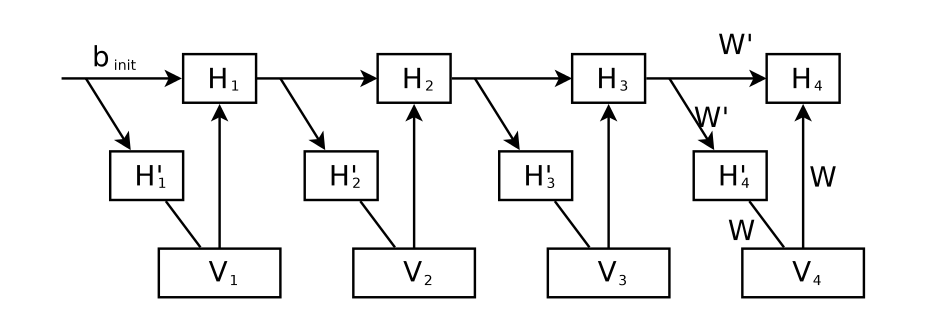
\includegraphics[scale=0.4]{Figures/RTRBM.png}
    \rule{35em}{0.5pt}
    \caption[RTRBM Graphical Model]{RTRBM Graphical Model}
    \label{fig:rtrbm}
\end{figure}

Boulanger-Lewandowski et al. change the RTRBM model to use a classical RNN to generate the biases for the RBM of the next time step (RNN-RBM \cite{boulanger2012modeling}): 
$$
\begin{array}{rcr}
    b_v^{(t)} & = & b_v + W_ {uv} u^{(t - 1)} \\
    b_h^{(t)} & = & b_h + W_{uh} u^{(t - 1)} \\
    u^{(t)} & = & tanh( b_u + W_{uu} u^{(t - 1)} + W_{vu}v^{(t)})
\end{array}
$$


\begin{figure}[htbp]
    \centering
    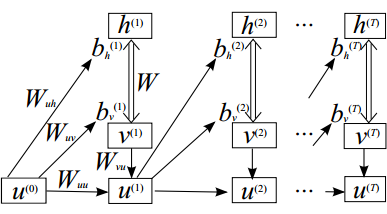
\includegraphics[scale=0.6]{Figures/RNNRBM.png}
    \rule{35em}{0.5pt}
    \caption[RNN-RBM Graphical Model]{RNN-RBM Graphical Model}
    \label{fig:rtrbm}
\end{figure}

This model was applied to the music score datasets and achieved the best results. However the model were not used for music generation specifically and this will be the focus of this project.

\section{Training Restricted Boltzman Machines unsing constrastive divergence.}


    Training a RBM using stochastic gradient descent requires to evaluate the log-likelihood gradient. However, it is difficult to determine the gradient analytically, and it becomes infeaseable even for a small RBM as it involves the computation of an expectation term over all input layer configuration :

From the Energy function of the RBM :
$$ E(v, h) = -a ^\top v - b^\top h - h^\top W v$$
we can conduct the following calculation 

\begin{figure}[htbp]
    \centering
    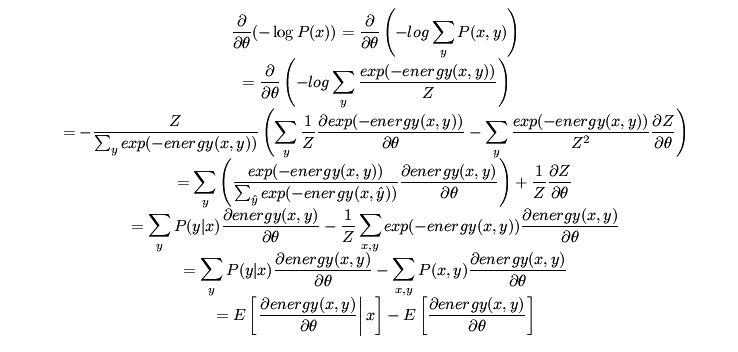
\includegraphics[scale=0.6]{Figures/calculation_cd.png}
    \rule{35em}{0.5pt}
    \caption[CD calculaiton]{CD calculation}
    \label{fig:calc_cd}
\end{figure}

So in the end, evaluating the negative log likelihood gradient of P consist of 2 terms : a positive contribution that lower the energy of the observed data, and a negative term that increase the energy of all the inputs.

In order to evaluate the gradient, Gibbs sampling is used in place of the expectation calculation. Gibbs sampling consist of running a Markov chain, using Gibbs step as the transition step. 

\begin{figure}[htbp]
    \centering
    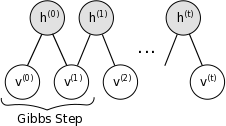
\includegraphics[scale=0.6]{Figures/gibbs_sampling.png}
    \rule{35em}{0.5pt}
    \caption[Gibbs sampling]{Gibbs Sampling}
    \label{fig:gibbs_sampling}
\end{figure}

Gibbs step : 

$$h^{(n+1)} \sim sigm(W^\top v^{(n)} + b )$$
$$v^{(n+1)} \sim sigm(W h^{(n+1)} + a )$$

In practice, the convergence of the sampling is not necessary and only k-steps are used (for Contrastive Divergence (CD-k)), and even that taking $k=1$ is works well.
In order to train a RBM as part of a bigger model (RTRBM, RNN-RBM), Gibbs sampling is used to create a specific instance of the RBM for which it is possible to obtain a gradient (using the samples instead of the expectation), it is then possible to use this gradient as part of the calculation for a stochastic gradient descent on the whole model.
